\section{Overview}
\label{sec:overview}

We now present an overview of our hardware approach for improving system performance by reducing or eliminating the overheads of sparse data computations in DNN training. Our technique comprises of extensions to the processor and memory systems that enable more efficient handling of zero data values and associated computations.  

\subsection{Processor Optimizations}
Our processor optimizations are based on the observation that the results of addition and multiplication operations---the core part of DNN training kernels---can be determined without performing the operation if one of the input operands is a zero.  We refer to instructions that perform these arithmetic operations with at least one zero-value input operand as ``zero-optimizable'' instructions.  In modern out-of-order processor pipelines, a zero-optimizable in the instruction queue presents a number of optimization opportunities because its result and side effects can sometimes be determined once the zero input operand becomes available. In particular, a zero-optimizable instruction could render some data dependencies and pipeline stages redundant, making it possible to non-speculatively issue or commit instructions earlier than normal or even squash instructions. We discuss these optimization opportunites in more details below using the DNN training code snippets in Figure~\ref{fig:gradient_code} to motivate the ideas.  Figure~\ref{fig:gradient_code}(a)  shows source code for error gradient computation, while Figure~\ref{fig:gradient_code} (b) shows the inner loop using sample machine instructions.  In the discussion below, we  assume that R$0$, which corresponds to errors[i] in the source code,  is zero in the loop. 

\subsubsection{Early Instruction Issue/Commit.}  First, a zero-optimizable instruction can be issued once the zero operand is available if the zero makes other operands redundant.  For example, I$4$ is a zero-optimizable instruction which can be issued early becaue it is a multiplication and the zero value of R$0$ makes R$2$ redundant.  Second, a zero-optimizable instruction could be committed early if the zero input determines its results and side effects. This is the case for I$4$. Early issue and commit of zero-optimizable instructions can reduce pressure on processor resources and wait times of data dependent instructions, such as I$5$, since the dependencies are satisfied sooner. 

\subsubsection{Instruction Squashing.} A zero-optimizable instruction can be squashed in the instruction queue if a zero input operand makes it an identity function and thus redundant. For this reason, I$5$ can be quashed since it is an addition and R$2$ is zero. Since a squashed instruction can make redundant other instructions that it depends on (producers) and that depend on it (consumers),  quashed zero-optimized instruction can make dependent instructions redundant as well.  For example, I$6$ is redundant and can be squashed since it is effectively a silent store. 
 



\begin{comment}
\begin{figure}[!t]
\centering
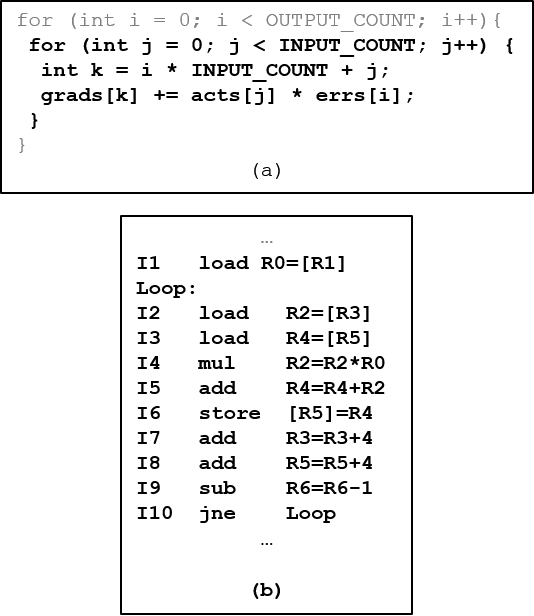
\includegraphics[width=2.4in]{Figures/gradient_code.png}
\caption{(a) Source code for computing error gradients and (b) corresponding machine instructions of inner loop.}
\label{fig:gradient_code}
\end{figure}
\end{comment}

\begin{figure*}
\centering
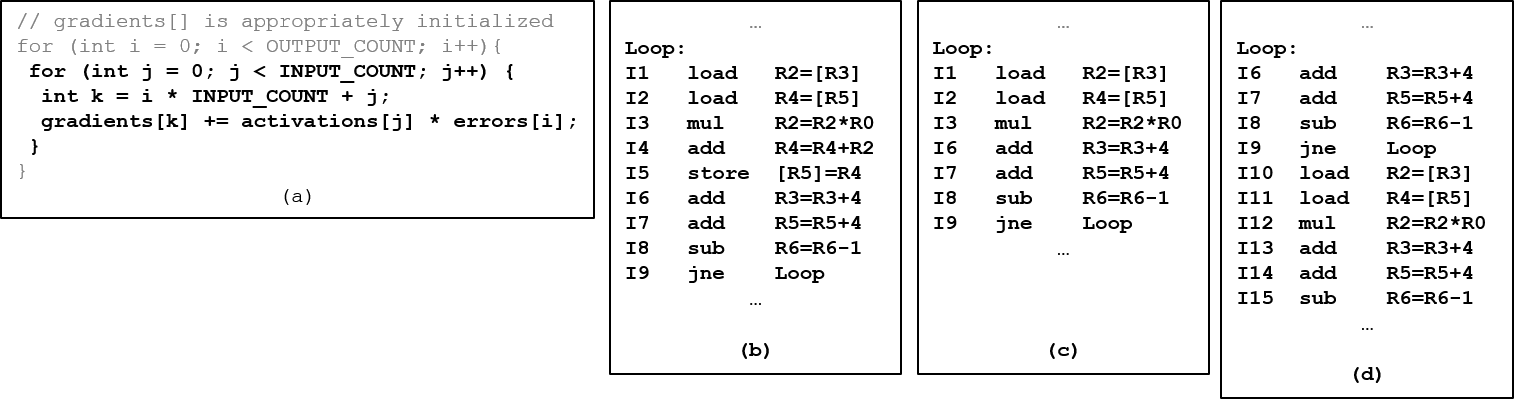
\includegraphics[width=1.9\columnwidth]{Figures/gradient_code_opt.png}
\caption{(a) Source code for computing error gradients, (b) machine code of inner loop, (c) optimized code after basic instruction quashing, and (d) optimized code after advanced instruction quashing.}
\label{fig:gradient_code}
\end{figure*}


\subsection{Memory System Optimizations}


 
 
